\section{Speeded Up Robust Features}
Speeded Up Robust Features (SURF) is a local feature transformation algorithm proposed by Herbert Bay, Tinne Tuytelaars, and Luc Van Gool in 2006 \cite{Bay2006}. Compared to SIFT \cite{Lowe1999}, the authors claim the SURF detector and descriptor to be faster and more robust against various image transformations.

\subsection{Key-point Detection}
The SURF key-point detection is based on the determinant of the Hessian matrix. Let us consider an input image $I_{img}(x,y)$ and the scale-space representation of the image
\begin{equation}
    L(x, y,\sigma) =  G(x,y,\sigma)*I_{img}(x,y),
\end{equation}
where $G(x,y,\sigma)$ is the Gaussian kernel defined in \eqref{eq:Gaussian_kernel}.

The Hessian matrix at scale $\sigma$ is defined as
\begin{equation}
    \mathcal{H}(x, y, \sigma) =
    \begin{bmatrix}
        L_{xx}(x, y, \sigma) & L_{xy}(x, y, \sigma)\\
        L_{xy}(x, y, \sigma) & L_{yy}(x, y, \sigma)
    \end{bmatrix},
\end{equation}
where $L_{xx}(x, y, \sigma)$, $L_{xy}(x, y, \sigma)$, and $L_{yy}(x, y, \sigma)$ are the second-order derivatives of the scale-space representation of the image at a point $(x, y)$.

The SURF authors decided to approximate the second order derivatives of Gaussian filter with box filters (shown in \figref{fig:Gauss_box_y}). Because the property of Gaussian filter, that no new structures can appear while going to a lower resolution, has been shown not to apply in 2D case \cite{Koenderink1984}. Box filters allow for the use of integral images, which reduces the computational complexity.

\begin{figure}
    \centering
    \begin{subfigure}{0.24\textwidth}
        \centering
        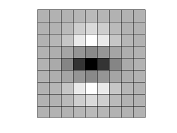
\includegraphics[width=\textwidth]{Figures/surf/y_gauss.png}
        \label{fig:y_gauss}
    \end{subfigure}
    \begin{subfigure}{0.24\textwidth}
        \centering
        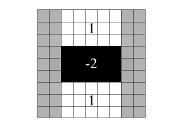
\includegraphics[width=\textwidth]{Figures/surf/y_box.png}
        \label{fig:y_box}
    \end{subfigure}
    \caption[Gaussian second-order derivative in the $y$-direction and its approximation using box filters]{Gaussian second order derivative in the $y$-direction and its approximation using box filters \cite{Bay2006}.}
    \label{fig:Gauss_box_y}
\end{figure}

Let us denote the approximations by $D_{xx}$, $D_{xy}$, and $D_{yy}$. The relative weights in the calculation of determinant of Hessian need to be weighted by $0.9$, which yields
\begin{equation}
    \text{det}(\mathcal{H}) = D_{xx} * D_{yy} - (0.9 * D_{xy})^{2}.
\end{equation}

Due to the use of box filters and integral images, any size of the box filter can be applied to the original image at the same speed directly. Therefore, the scale space is created by the use of up-scaled filters of sizes $9\times9$, $15\times15$, $21\times21$, $27\times27$, etc. For each octave, the difference between filter sizes is doubled (from $6$ to $12$ to $24$).

As the box filter layout remains the same, the corresponding Gaussian filter scales accordingly. The $9\times9$ box filter corresponds to a Gaussian filter with the scale $\sigma = 1.2$. Based on the definition of the process, we can calculate the corresponding Gaussian filter scale for each box filter size.

To select the key-points, non-maximum suppression in the $3\times3\times3$ neighborhood of each point is applied. Afterwards, the maxima of the determinant of the Hessian matrix are interpolated the same way as in the SIFT algorithm (using quadratic Taylor expansion).

\subsection{Key-point Description}
At first, we need to ensure the descriptor's invariance to rotation. For every key-point, we calculate the Haar-wavelet responses in the $x$ and the $y$ direction in a circular neighborhood of $6s$, where $s$ is the Gaussian filter scale at which the key-point was found. Integral images are used for speeding up the process.

The wavelet responses are weighted with a Gaussian($\sigma = 2.5 s$) centered at the key-point. The weighted responses are represented as vectors in a space with the $x$ response being a vector along the $x$-axis, and the $y$ response being a vector along the $y$-axis. All the vectors within a sliding window of $\frac{\pi}{3}$ are summed and the longest of the vector is selected as the key-point orientation.

An example of key-points and their orientation, found by OpenCV SURF implementation, is presented in \figref{fig:surf_example}.
\begin{figure}[ht!]
    \centering
    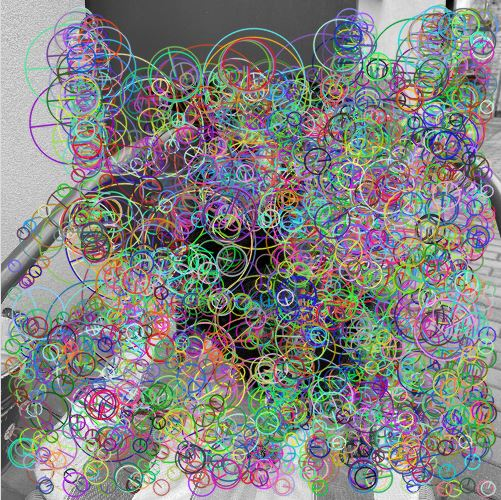
\includegraphics[width=0.60\textwidth]{Figures/surf/surf_example.jpg}
    \caption[SURF key-points and their orientation from an image of a dog]{SURF key-points and their orientation from an image of a dog.}
    \label{fig:surf_example}
\end{figure}

The descriptor is constructed from a square window the size of $20s$ around a key-point. The window is subsequently rotated along with the key-point orientation. Afterwards, this window is divided into $16$ ($4\times4$) square sub-windows. In each sub-window, the features are calculated using $5\times5$ regularly spaced sample points. From these sample points, we calculate the Haar wavelet responses in the horizontal and the vertical direction, where \say{horizontal} and \say{vertical} are defined in relation to the key-point orientation. The responses are weighted with a Gaussian ($\sigma = 3.3s$) centered at the key-point.

Let us call the horizontal responses $d_x$ and the vertical responses $d_y$. Over each sub-window, we denote the sum of the responses $\sum d_x$ and $\sum d_y$, and the sum of absolute values of the responses $\sum |d_x|$ and $\sum |d_y|$. The behavior of these values for different image patterns can be seen in \figref{fig:surf_descriptor}. Combining $\sum d_x$, $\sum d_y$, $\sum |d_x|$, and $\sum |d_y|$ for each of the $16$ sub-window into a vector, we get a descriptor of length $64$.

\begin{figure}
    \centering
    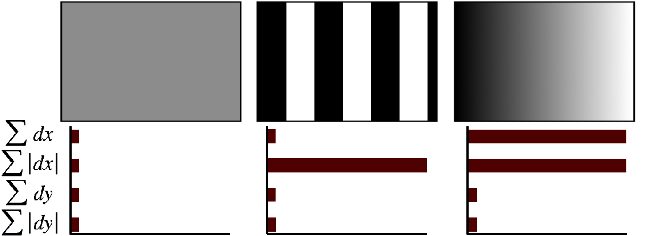
\includegraphics[width=0.8\textwidth]{Figures/surf/surf_descriptor.png}
    \caption[Behaviour of SURF descriptor for different image patterns]{Behaviour of SURF descriptor for different image patterns \cite{Bay2006}.}
    \label{fig:surf_descriptor}
\end{figure}
